\section{Introduction}\label{sec:introduction}
  The Secure Hashing Algorithm (SHA) family of cryptography is widely used as a means of providing increased security through generating/verifying digital signatures, deriving keys, and generating pseudorandom bits. (NIST: https://csrc.nist.gov/publications/detail/fips/202/final)  
  The structure and computations of these algorithms is defined by NIST in mathematical specifications.  
  Because these specifications are just figures on a page, any assurance of correctness of an algorithm’s implementation is dependent on a visual review of the code coupled with a small sampling of test vectors.
  
  The reliability of this correctness check is often weakened because of the difficulty of performing that visual review.  
  Many implementations of the SHA algorithms go through major rewrites and optimizations which make visual inspection of the code nearly impossible. (Not sure if that’s too strong a claim).
  This work bridges that gap between optimized c code, and the NIST standard.
  
%%\onecolumn
\begin{figure*}[ht]
  \centering
  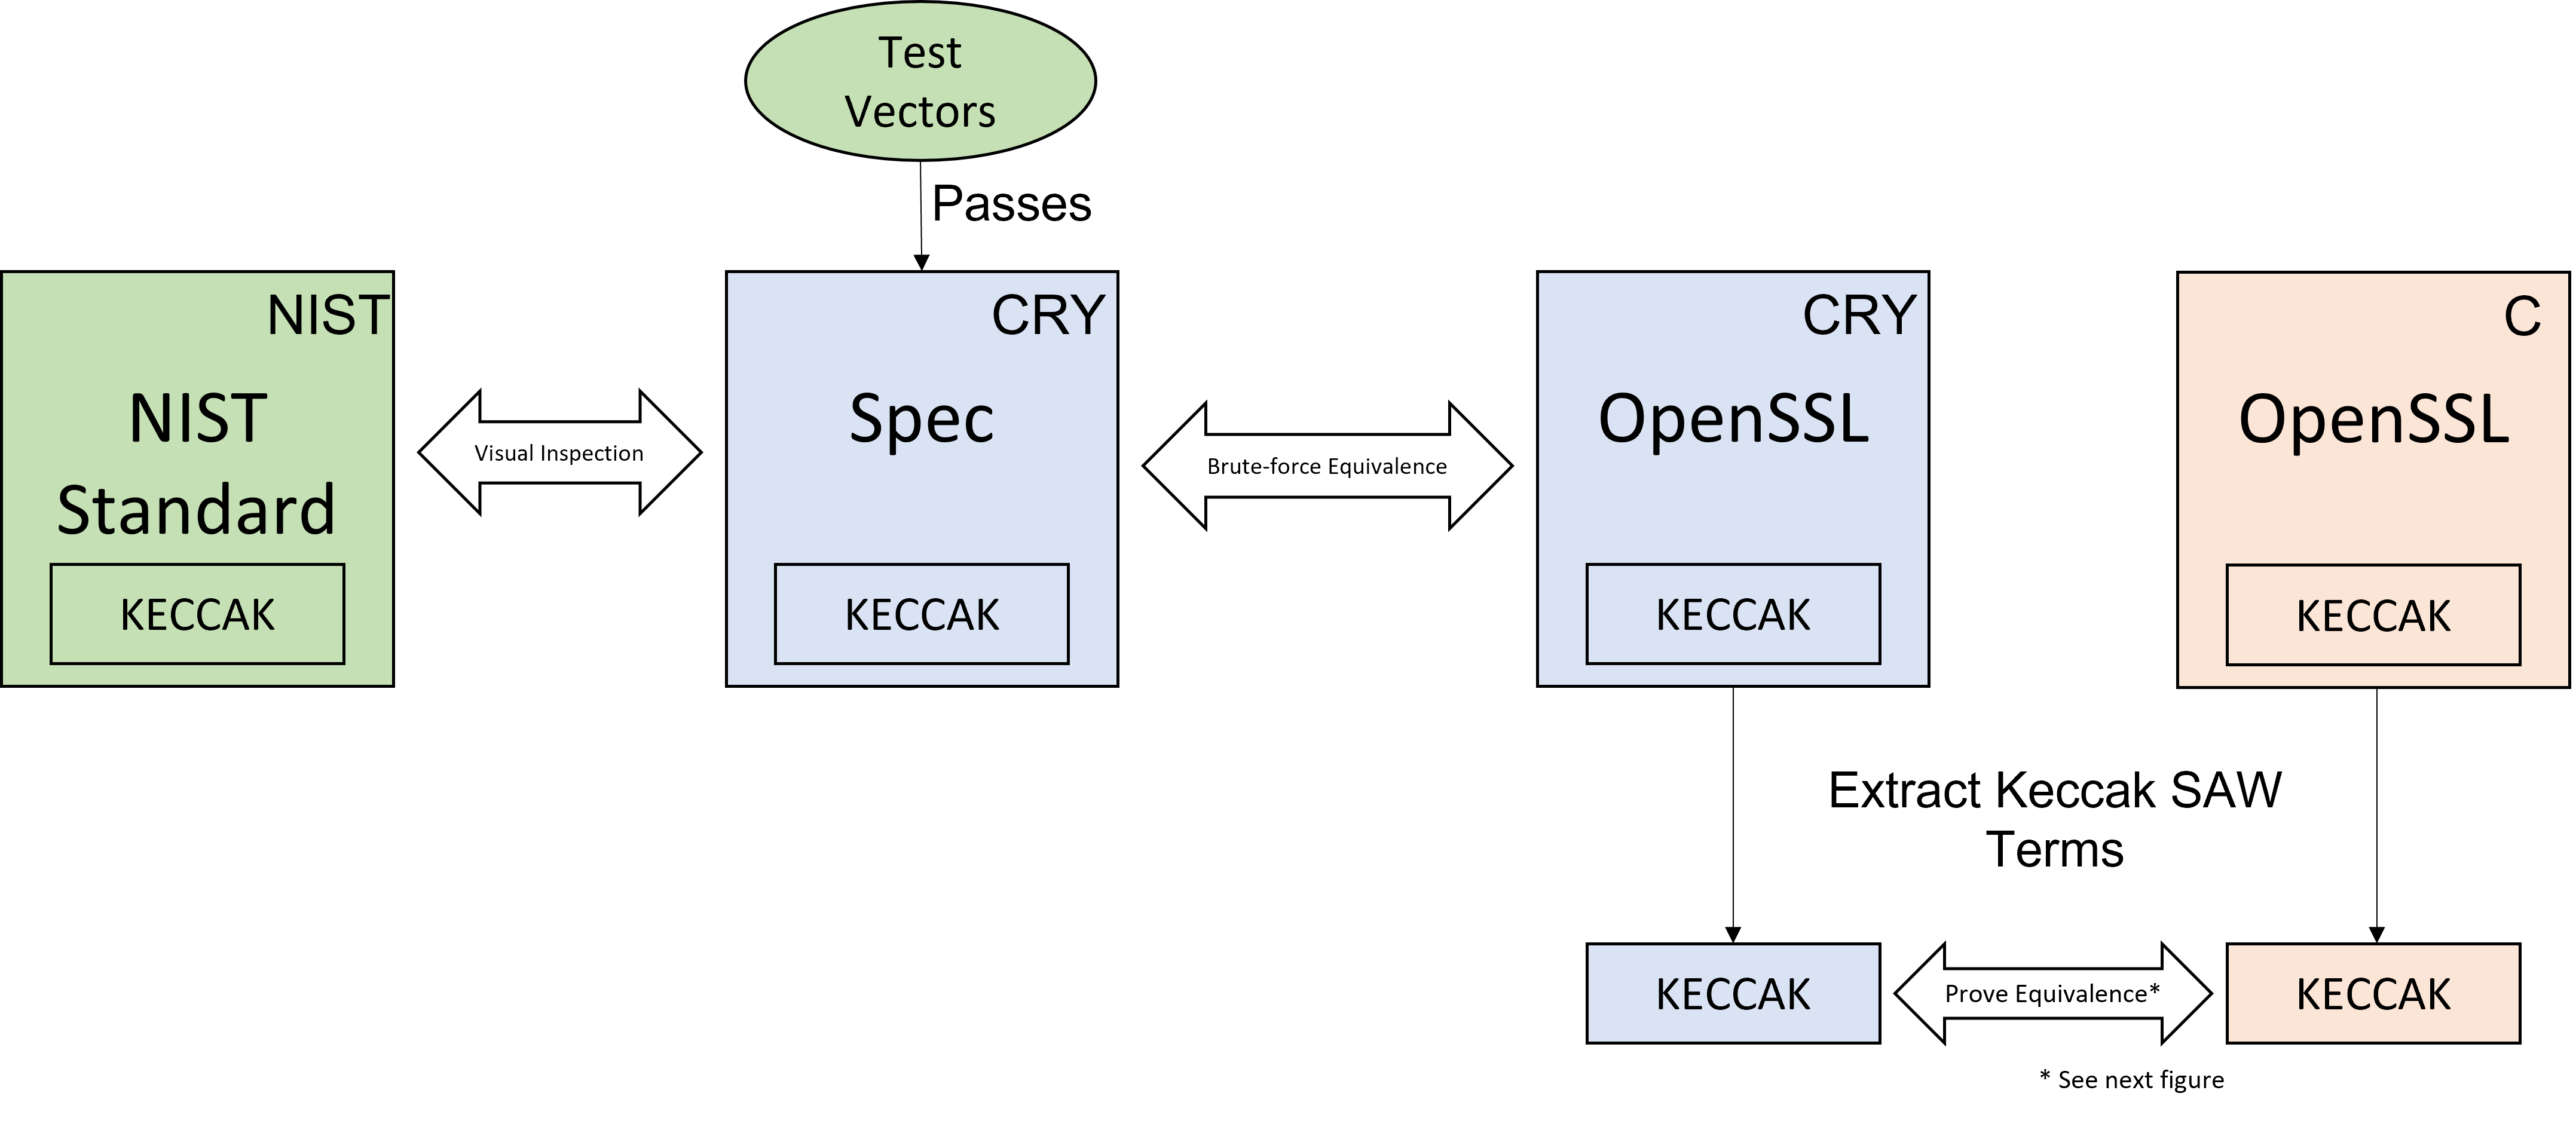
\includegraphics[width=\linewidth]{img/proof.png}
  
  \caption{SHA3 Keccak Proof Structure}
  \label{fig:proofStructure}
  
\end{figure*}
%%\twocolumn

\noindent \textbf{Contributions}:
This paper details the following contributions.
\begin{compactitem}
  \item  A Cryptol specification for \texttt{SHA3} that directly corresponds to the \texttt{FIPS} 202 specification and passes the test vectors provided by the same specification.
  \item A Cryptol specification based on the OpenSSL implementation of \texttt{SHA3} that uses a reordered state vector and precomputed tables in Keccak for performance gains and passes test vectors
  \item A \texttt{SAW} proof that the \texttt{FIPS} 202 specification is equivalent to the OpenSSL specification
  \item A \texttt{SAW} proof that the OpenSSL Keccak specification is equivalent to the OpenSSL C-implementation of the same function for all possible state vector input
  \item Early evidence that modular cryptographic specifications such as \texttt{SHA3} lend themselves to efficient \texttt{SAW} verification against C implementations as opposed to flattened specifications such as \texttt{SHA2} 
\end{compactitem}

\noindent \textbf{Limitations}
\begin{compactitem}
  \item Visual inspection and limited test vectors for (1) and (2)
  \item Only provide proof certificates for message sizes of X to Y for digest sizes of … for (3)
  \item Visual inspection only for anything above Keccak for (3) in OpenSSLs C-code
\end{compactitem}

\subsection{Related Work}
  Previously, Galois’ Inc. worked with Amazon to prove out parts of Amazon’s s2n HMAC code to the NIST specification.  
In their work they stubbed out use of the SHA2 algorithm because their HMAC allows for customization of the algorithm type and implementation.

The work by Decker et. al, extended on Galois' work by choosing a single SHA2 implementation to prove out.  
They chose OpenSSL’s SHA 256 implementation, as that is a commonly used library (and one that is usable in s2n).  
They were able to prove out the inner hash computations of that implementation using a methodology of compositional proofs to do so.  
They were also able to connect up their proof with the code used by Galois’ to stub out the SHA2 algorithm, which implies that the functional equivalence property established with the OpenSSL code applies to Galois' Cryptol implementation as well.  
Their work showed the viability and limitations of creating proofs of functional equivalence for legacy cryptographic implementations.



\subsection{SHA 3}
This work shows that this same methodology can be extended to modern cryptographic algorithms.
The SHA 3 family of algorithms is defined by NIST in the FIPS 202 publication.
It specifies a block hashing algorithm, Keccak, that is used by each of the different SHA and SHAKE algorithms.
In comparison to the SHA 2 family of algorithms, Keccak features significantly more complex and robust computations.
This increase in computation was of interest, because it presses the limits of SAW's capabilities.

\subsection{Results}
This work shows a complete proof of functional equivalence from a verified implementation of the NIST standard to OpenSSL's C code for the Keccak function.
In doing so, it shows SAW's ability to stand up against more difficult computations.
It also provides insights into using Cryptol's functional nature to further simplify the step of visually verifying Cryptol code to the NIST standard.

Because of how NIST defines the standard, the keccak function is used for each digest size of the SHA3 algorithm, with the only significant differences being in the padding/sponging parts of the algorithm, which falls outside this work's scope.
This means that the proof of correctness for this function extends usefulness beyond just the SHA3-256 level which we focused on.
In our repository, we wrote the Cryptol specification to be able to run any of the SHA3 family of algorithms using the same keccak.
A simple extension of this work would be to take that already created and verified Cryptol specification, and prove it up against OpenSSL's slightly modified keccak versions.